\section{Zobecněné lineární regresní modely. Modely pro binární, multinomickou a čítací závisle proměnnou}

\subsection{Motivace}

Klasická lineární regrese je vhodná hlavně tehdy, když je závisle proměnná přibližně spojitá a není omezena
na malý počet hodnot. Pro mnoho ekonomických a sociálních dat to ale neplatí.

Typické příklady:
\begin{itemize}
    \item binární proměnná: zaměstnaný / nezaměstnaný,
    \item kategoriální proměnná: volba značky, politické strany nebo dopravního prostředku,
    \item čítací proměnná: počet návštěv lékaře, počet nákupů, počet nehod,
    \item cenzorovaná proměnná: mzda oříznutá shora nebo výdaje s mnoha nulami.
\end{itemize}

V takových situacích se používají zobecněné lineární modely nebo modely s omezenou závisle proměnnou.

\subsection{Obecný rámec GLM}

U zobecněného lineárního modelu rozlišujeme:
\[
\mu_i=\mathrm{E}(y_i|x_i),
\]
a lineární prediktor:
\[
\eta_i=x_i^\top\beta.
\]

GLM spojuje střední hodnotu $\mu_i$ s lineárním prediktorem pomocí link funkce:
\[
g(\mu_i)=x_i^\top\beta.
\]

Kde:
\begin{itemize}
    \item $g(\cdot)$ je link funkce,
    \item $\mu_i$ je podmíněná střední hodnota,
    \item $x_i^\top\beta$ je lineární index.
\end{itemize}

\paragraph{Intuice.}
Nechceme nutně modelovat $y$ přímo jako lineární funkci $x$. Místo toho modelujeme vhodnou transformaci
střední hodnoty. Například u binární proměnné nechceme, aby predikovaná pravděpodobnost byla menší než 0
nebo větší než 1. Proto použijeme link funkci, která to zajistí.

Parametry se většinou odhadují metodou maximální věrohodnosti:
\[
\hat\beta = \arg\max_{\beta}\ell(\beta).
\]

\subsection{Binární závisle proměnná}

Binární proměnná nabývá pouze hodnot:
\[
y_i\in\{0,1\}.
\]

Například:
\[
y_i=
\begin{cases}
1, & \text{pokud je osoba nezaměstnaná},\\
0, & \text{jinak}.
\end{cases}
\]

Cílem je modelovat pravděpodobnost:
\[
p_i=P(y_i=1|x_i).
\]

\subsection{Lineární pravděpodobnostní model}

Nejjednodušší model pro binární $y$ je lineární pravděpodobnostní model:
\[
P(y_i=1|x_i)=\beta_0+\beta_1x_{i1}+\cdots+\beta_kx_{ik}.
\]

Tedy:
\[
p_i=x_i^\top\beta.
\]

\paragraph{Interpretace.}
Koeficient $\beta_j$ říká, o kolik se změní pravděpodobnost úspěchu při jednotkové změně $x_j$:
\[
\Delta P(y=1|x)=\beta_j\Delta x_j.
\]

Pokud $\beta_j=0.05$, pak jednotkové zvýšení $x_j$ zvyšuje pravděpodobnost o 0.05, tedy o 5 procentních
bodů.

\subsubsection{Výhody LPM}

\begin{itemize}
    \item jednoduchý odhad pomocí OLS,
    \item jednoduchá interpretace koeficientů,
    \item dobrý základní model pro rychlou analýzu.
\end{itemize}

\subsubsection{Nevýhody LPM}

LPM má dvě hlavní nevýhody.

Za prvé, predikované pravděpodobnosti mohou být mimo interval $[0,1]$:
\[
\hat p_i < 0
\quad \text{nebo} \quad
\hat p_i > 1.
\]

To nedává smysl, protože pravděpodobnost nemůže být záporná ani větší než jedna.

Za druhé, model je automaticky heteroskedastický. Pro binární proměnnou platí:
\[
\mathrm{Var}(y_i|x_i)=p_i(1-p_i).
\]

Protože $p_i$ závisí na $x_i$, závisí na $x_i$ i rozptyl.

\paragraph{Řešení.}
U LPM je vhodné používat robustní standardní chyby. Ještě lepší je často použít logit nebo probit.

\subsection{Logit a probit}

Logit a probit modelují pravděpodobnost pomocí nelineární funkce:
\[
P(y_i=1|x_i)=F(x_i^\top\beta).
\]

Funkce $F$ zajišťuje, že výsledek vždy leží mezi 0 a 1:
\[
0<F(x_i^\top\beta)<1.
\]

\subsubsection{Logit}

U logitu:
\[
F(z)=\Lambda(z)=\frac{1}{1+e^{-z}}.
\]

Tedy:
\[
P(y_i=1|x_i)
=
\frac{1}{1+e^{-x_i^\top\beta}}.
\]

\begin{figure}[htbp]
  \centering
  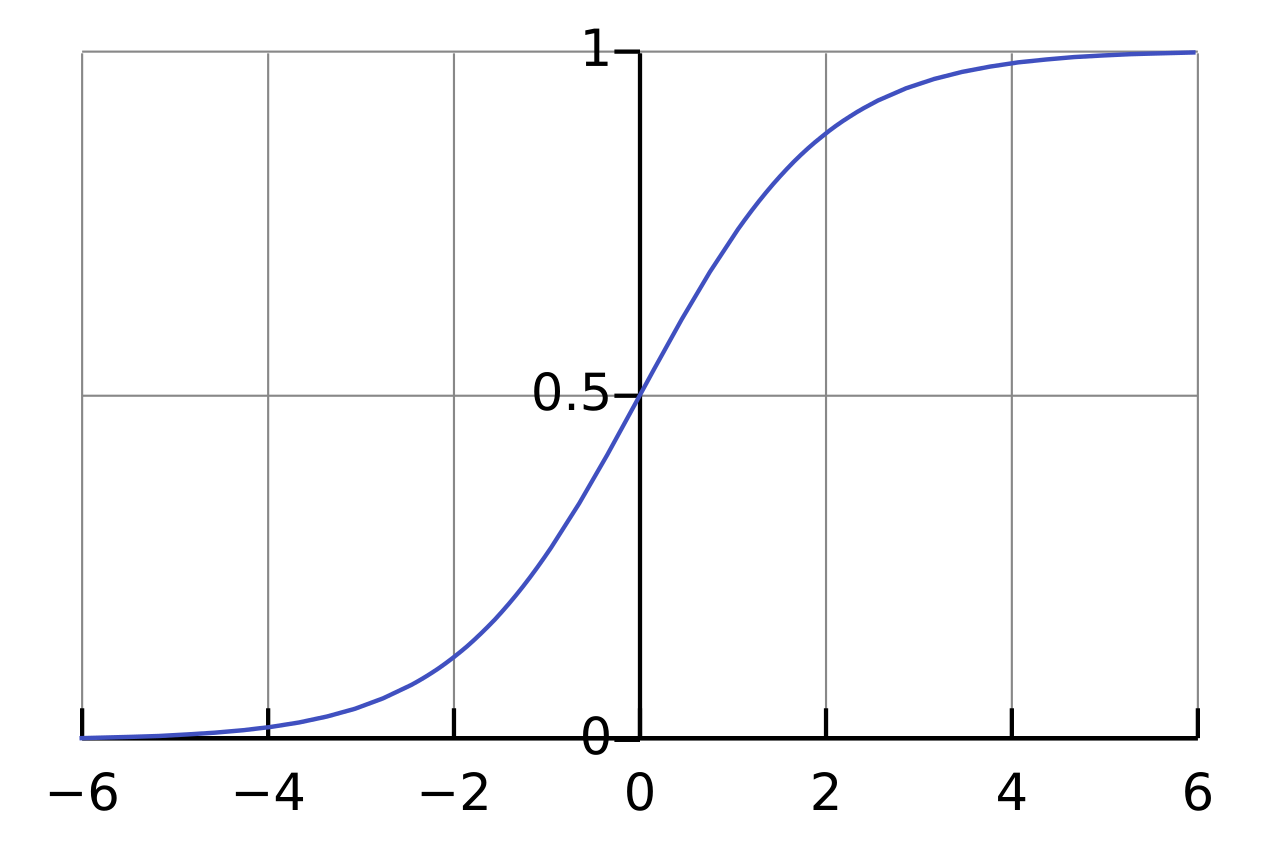
\includegraphics[width=0.72\linewidth]{assets/images/zobecnene-linearni-modely/logistic-curve.png}
  \caption[Logistická funkce]{Logistická funkce používaná v logitu. Popis obrázku: S-křivka převádí
  lineární index $x_i^\top\beta$ na hodnotu mezi 0 a 1, tedy na predikovanou pravděpodobnost úspěchu.
  Největší změna pravděpodobnosti nastává kolem středu křivky, kde je $p$ blízko 0.5. Zdroj obrázku:
  Qef, \href{https://commons.wikimedia.org/wiki/File:Logistic-curve.svg}{Wikimedia Commons},
  licence public domain.}
  \label{fig:logistic-curve}
\end{figure}

\subsubsection{Probit}

U probitu:
\[
F(z)=\Phi(z),
\]
kde $\Phi$ je distribuční funkce standardního normálního rozdělení.

\[
P(y_i=1|x_i)=\Phi(x_i^\top\beta).
\]

\subsection{Latentní interpretace logitu a probitu}

Logit a probit lze chápat přes latentní, tedy nepozorovanou, proměnnou:
\[
y_i^*=x_i^\top\beta+u_i.
\]

Pozorujeme pouze:
\[
y_i=
\begin{cases}
1, & y_i^*>0,\\
0, & y_i^*\leq 0.
\end{cases}
\]

\paragraph{Intuice.}
Například rozhodnutí stát se podnikatelem závisí na nepozorované bilanci výhod a nevýhod.
Pokud latentní užitek podnikání překročí určitou hranici, pozorujeme $y=1$.

Rozdíl mezi logitem a probitem je v předpokladu o rozdělení chyby $u_i$:
\begin{itemize}
    \item logit používá logistické rozdělení,
    \item probit používá normální rozdělení.
\end{itemize}

V praxi často dávají podobné výsledky.

\subsection{Log-likelihood u binárního modelu}

Protože $y_i$ je binární, příspěvek jednoho pozorování k věrohodnosti lze zapsat jako:
\[
P(y_i|x_i)
=
p_i^{y_i}(1-p_i)^{1-y_i}.
\]

Log-likelihood:
\[
\ell(\beta)
=
\sum_{i=1}^n
\left[
y_i\log(p_i)+(1-y_i)\log(1-p_i)
\right].
\]

Kde:
\[
p_i=F(x_i^\top\beta).
\]

Odhad $\hat\beta$ maximalizuje tuto log-likelihood funkci.

\subsection{Interpretace logitu}

Logit lze přepsat pomocí odds:
\[
odds = \frac{p}{1-p}.
\]

Odds říkají, kolikrát je úspěch pravděpodobnější než neúspěch.

Logit model:
\[
\log\left(\frac{p_i}{1-p_i}\right)
=
x_i^\top\beta.
\]

Koeficient $\beta_j$ tedy přímo nemění pravděpodobnost, ale logaritmus odds.

Po exponenciaci:
\[
e^{\beta_j}
\]
dostáváme odds ratio.

\paragraph{Interpretace odds ratio.}
Pokud:
\[
e^{\beta_j}=1.2,
\]
pak jednotkové zvýšení $x_j$ násobí odds faktorem 1.2, tedy zvyšuje odds o 20\%.

\paragraph{Pozor.}
To neznamená, že pravděpodobnost vzroste o 20 procentních bodů. V logitu se efekt na pravděpodobnost mění
podle hodnot ostatních proměnných.

\subsection{Marginální efekty}

U logitu a probitu nejsou koeficienty přímo marginální efekty na pravděpodobnost.

Pro spojitou proměnnou:
\[
\frac{\partial p_i}{\partial x_{ij}}
=
f(x_i^\top\beta)\beta_j.
\]

Kde $f$ je hustota odpovídající distribuční funkci $F$.

U logitu konkrétně:
\[
\frac{\partial p_i}{\partial x_{ij}}
=
p_i(1-p_i)\beta_j.
\]

\paragraph{Důsledek.}
Stejný koeficient $\beta_j$ může znamenat různě velkou změnu pravděpodobnosti pro různé osoby. Největší
efekty bývají kolem $p=0.5$, menší efekty u pravděpodobností blízko 0 nebo 1.

\subsubsection{Average marginal effect}

Často se reportuje průměrný marginální efekt:
\[
AME_j
=
\frac{1}{n}
\sum_{i=1}^n
f(x_i^\top\hat\beta)\hat\beta_j.
\]

\subsubsection{Dummy proměnná}

U dummy proměnné se nepočítá derivace, ale diskrétní změna:
\[
F(\hat\eta_i|x_j=1)-F(\hat\eta_i|x_j=0).
\]

Tedy rozdíl predikované pravděpodobnosti při změně dummy proměnné z 0 na 1.

\subsection{Hodnocení binárního modelu}

U binárních modelů klasické $R^2$ nemá stejnou interpretaci jako v OLS.

Možnosti hodnocení:
\begin{itemize}
    \item procento správně klasifikovaných pozorování,
    \item log-likelihood,
    \item pseudo-$R^2$,
    \item ROC křivka a AUC,
    \item citlivost a specificita.
\end{itemize}

Pro klasifikaci často používáme pravidlo:
\[
\hat y_i=
\begin{cases}
1, & \hat p_i>0.5,\\
0, & \hat p_i\leq 0.5.
\end{cases}
\]

\paragraph{Pozor.}
Hranice 0.5 nemusí být vždy vhodná. Pokud jsou náklady na falešně pozitivní a falešně negativní chybu
odlišné, volíme jiný práh.

ROC křivka ukazuje, jak se mění citlivost a falešně pozitivní míra při různých klasifikačních prazích.
Jeden bod na ROC křivce odpovídá jednomu konkrétnímu prahu: na ose \(x\) je false positive rate a na
ose \(y\) true positive rate. AUC shrnuje schopnost modelu odlišit jedničky od nul do jednoho čísla.
Neříká ale, zda jsou predikované pravděpodobnosti dobře kalibrované ani jaký práh je nejlepší pro
konkrétní business situaci.

\begin{figure}[htbp]
  \centering
  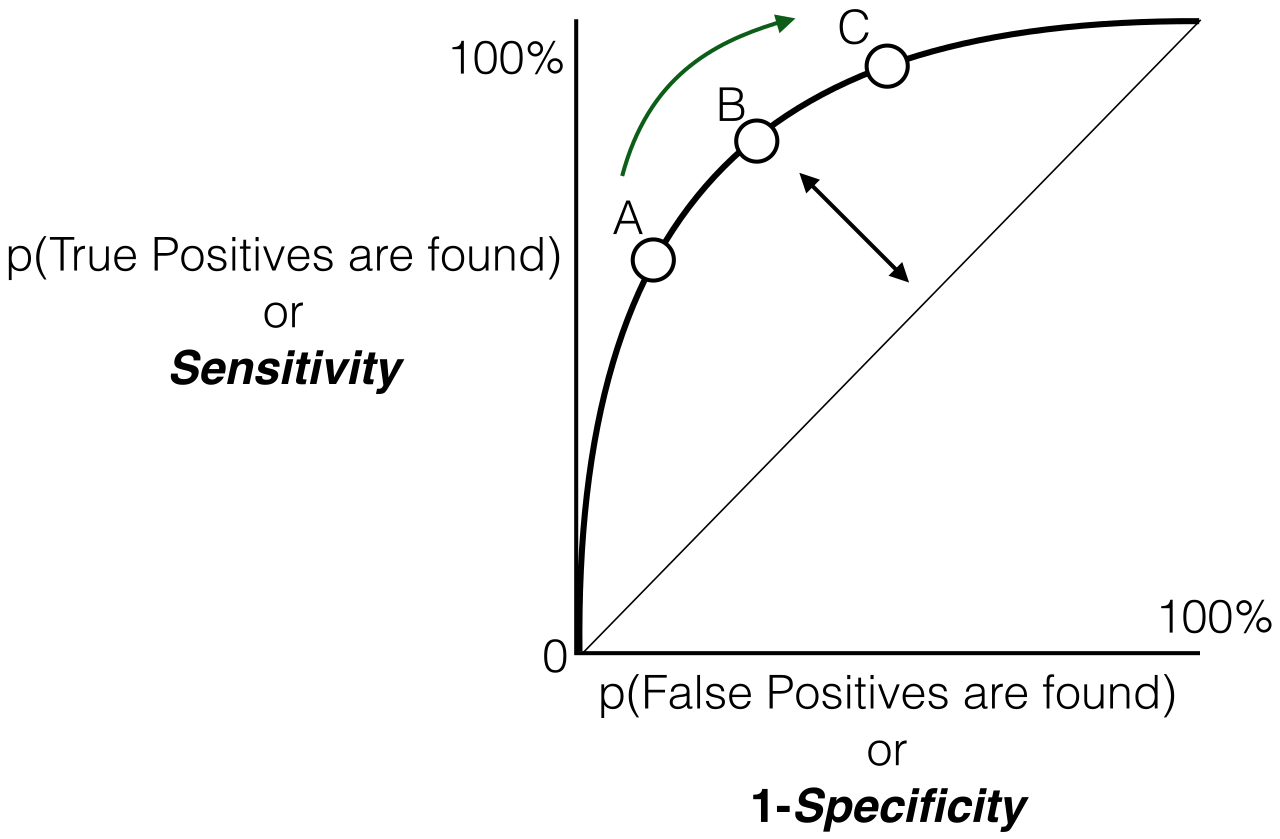
\includegraphics[width=0.76\linewidth]{assets/images/zobecnene-linearni-modely/roc-curve.png}
  \caption[ROC křivka]{ROC křivka pro binární klasifikaci. Popis obrázku: osa $y$ zobrazuje citlivost
  neboli true positive rate, osa $x$ falešně pozitivní míru neboli $1-\text{specificity}$. Body na křivce
  odpovídají různým rozhodovacím prahům; křivka blíže levému hornímu rohu znamená lepší diskriminaci.
  Zdroj obrázku: Masato8686819,
  \href{https://commons.wikimedia.org/wiki/File:ROC\_curve.svg}{Wikimedia Commons},
  licence CC BY-SA 3.0.}
  \label{fig:roc-curve}
\end{figure}

\subsection{Ordinální závisle proměnná}

Ordinální proměnná má více kategorií, které mají přirozené pořadí.

Příklady:
\begin{itemize}
    \item dosažené vzdělání: základní, střední, vysoké,
    \item spokojenost: nespokojen, neutrální, spokojen,
    \item odpověď v dotazníku: rozhodně ne, spíše ne, spíše ano, rozhodně ano.
\end{itemize}

Modelujeme latentní proměnnou:
\[
y_i^*=x_i^\top\beta+u_i.
\]

Pozorované kategorie vznikají podle prahů:
\[
y_i=k
\iff
\alpha_{k-1}<y_i^*\leq \alpha_k.
\]

Pravděpodobnost kategorie:
\[
P(y_i=k|x_i)
=
F(\alpha_k-x_i^\top\beta)
-
F(\alpha_{k-1}-x_i^\top\beta).
\]

Pokud je $F$ logistická distribuční funkce, jde o ordinální logit. Pokud je $F$ normální distribuční funkce,
jde o ordinální probit.

\paragraph{Intuice.}
Vyšší hodnota latentní proměnné posouvá pozorování do vyšších kategorií.

\subsection{Multinomická závisle proměnná}

Multinomická proměnná má více kategorií bez přirozeného pořadí:
\[
y_i\in\{0,1,\ldots,J\}.
\]

Příklady:
\begin{itemize}
    \item volba politické strany,
    \item volba dopravního prostředku,
    \item volba značky produktu,
    \item volba studijního oboru.
\end{itemize}

Protože kategorie nejsou uspořádané, nemůžeme použít ordinální logit/probit.

\subsection{Latentní užitek}

U multinomických modelů se často používá interpretace přes latentní užitek:
\[
U_{ij}=x_i^\top\beta_j+u_{ij}.
\]

Jedinec $i$ si vybere alternativu s nejvyšším užitkem:
\[
y_i=j
\iff
U_{ij}>U_{ih}
\quad
\text{pro všechna } h\neq j.
\]

\paragraph{Intuice.}
Při volbě mezi autem, autobusem a vlakem má každá alternativa pro člověka určitý užitek. Vybere tu, která
má nejvyšší užitek.

\subsection{Multinomický logit}

Pravděpodobnost volby alternativy $j$:
\[
P(y_i=j|x_i)
=
\frac{\exp(x_i^\top\beta_j)}
{\sum_{h=0}^{J}\exp(x_i^\top\beta_h)}.
\]

Protože pravděpodobnosti se musí sečíst na 1 a model jinak není identifikovaný, jedna kategorie se volí
jako referenční:
\[
\beta_0=0.
\]

Potom:
\[
\log\left(
\frac{P(y_i=j|x_i)}
{P(y_i=0|x_i)}
\right)
=
x_i^\top\beta_j.
\]

\paragraph{Interpretace.}
Koeficienty se interpretují vzhledem k referenční kategorii. Pokud je referenční volba například autobus,
pak koeficient u auta říká, jak proměnná mění log-poměr pravděpodobnosti volby auta proti autobusu.

Po exponenciaci:
\[
e^{\beta_{jr}}
\]
dostáváme relative risk ratio pro kategorii $j$ vůči referenční kategorii.

\subsection{IIA předpoklad}

Multinomický logit má důležitý předpoklad:
\[
IIA = \text{independence of irrelevant alternatives}.
\]

Tento předpoklad říká, že poměr pravděpodobností dvou alternativ nezávisí na dalších dostupných
alternativách:
\[
\frac{P(y=j|x)}{P(y=k|x)}
\]
se nezmění přidáním nebo odebráním jiné alternativy.

\paragraph{Problém.}
Pokud jsou některé alternativy blízké substituty, IIA může být nerealistický. Například přidání druhého
velmi podobného autobusu by nemělo stejně ovlivnit poměr volby auta a původního autobusu jako přidání
zcela jiné alternativy.

\subsection{Multinomický probit}

Multinomický probit umožňuje korelaci mezi chybami jednotlivých alternativ. Díky tomu nevyžaduje IIA.

Výhody:
\begin{itemize}
    \item flexibilnější,
    \item realističtější u podobných alternativ.
\end{itemize}

Nevýhody:
\begin{itemize}
    \item výpočetně náročný,
    \item horší použitelnost při velkém počtu kategorií.
\end{itemize}

\subsection{Čítací závisle proměnná}

Čítací proměnná nabývá hodnot:
\[
y_i\in\{0,1,2,\ldots\}.
\]

Příklady:
\begin{itemize}
    \item počet návštěv lékaře za rok,
    \item počet absencí v práci,
    \item počet nehod v regionu,
    \item počet nákupů zákazníka,
    \item počet defektů ve výrobní dávce.
\end{itemize}

Použít klasickou lineární regresi může být nevhodné, protože:
\begin{itemize}
    \item může predikovat záporné počty,
    \item počty bývají nesymetrické,
    \item rozptyl často roste se střední hodnotou.
\end{itemize}

\subsection{Poissonův regresní model}

Základní model:
\[
Y_i|x_i \sim Poisson(\mu_i).
\]

Poissonovo rozdělení:
\[
P(Y_i=y_i|x_i)
=
\frac{e^{-\mu_i}\mu_i^{y_i}}{y_i!}.
\]

Podmíněná střední hodnota:
\[
\mathrm{E}(Y_i|x_i)=\mu_i.
\]

Poissonův model používá log link:
\[
\log(\mu_i)=x_i^\top\beta.
\]

Tedy:
\[
\mu_i=\exp(x_i^\top\beta).
\]

\paragraph{Proč log link?}
Exponenciální funkce je vždy kladná, takže model nikdy nepredikuje záporný očekávaný počet.

\begin{figure}[htbp]
  \centering
  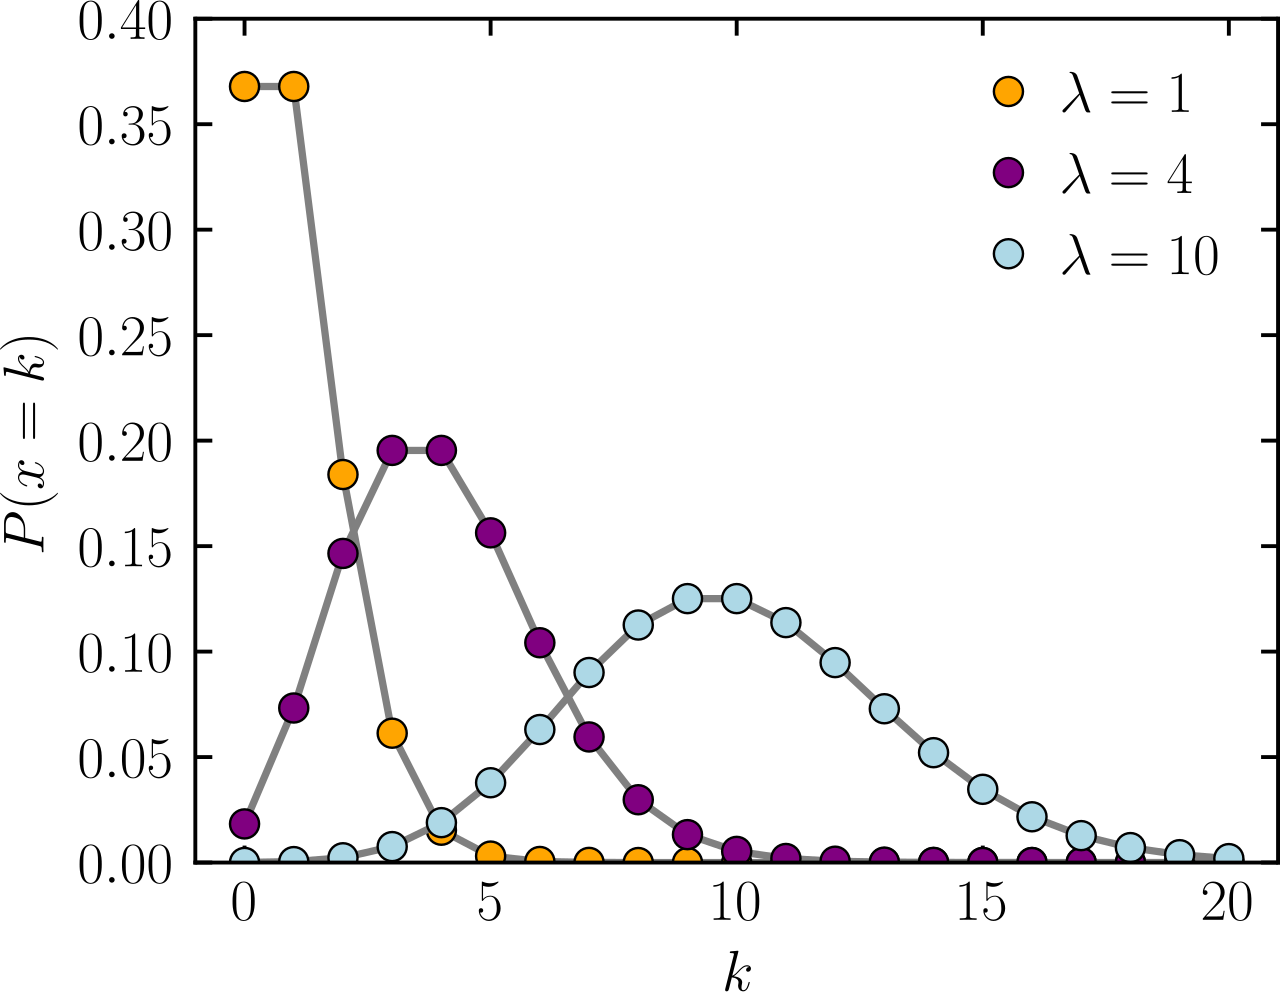
\includegraphics[width=0.76\linewidth]{assets/images/zobecnene-linearni-modely/poisson-pmf.png}
  \caption[Poissonovo rozdělení]{Pravděpodobnostní funkce Poissonova rozdělení pro různé hodnoty
  parametru $\lambda$. Popis obrázku: rozdělení je diskrétní, nabývá nezáporných celých hodnot a s rostoucí
  střední hodnotou se posouvá doprava. Právě proto se hodí pro modelování počtů událostí. Zdroj obrázku:
  Skbkekas, \href{https://commons.wikimedia.org/wiki/File:Poisson\_pmf.svg}{Wikimedia Commons},
  licence CC BY 3.0.}
  \label{fig:poisson-pmf}
\end{figure}

\subsection{Interpretace Poissonova modelu}

Protože:
\[
\mu_i=\exp(x_i^\top\beta),
\]
jednotková změna $x_j$ násobí očekávaný počet faktorem:
\[
e^{\beta_j}.
\]

Tento faktor se nazývá incidence rate ratio.

Procentní změna očekávaného počtu:
\[
100(e^{\beta_j}-1)\%.
\]

\paragraph{Příklad.}
Pokud:
\[
\beta_j=0.2,
\]
pak:
\[
e^{0.2}\approx 1.22.
\]
Jednotkové zvýšení $x_j$ zvyšuje očekávaný počet přibližně o 22\%.

\subsection{Marginální efekt v Poissonově modelu}

\[
\frac{\partial \mu_i}{\partial x_{ij}}
=
\beta_j\mu_i.
\]

To znamená, že absolutní změna očekávaného počtu závisí na aktuální úrovni $\mu_i$.

\paragraph{Intuice.}
Stejná procentní změna může znamenat malý absolutní rozdíl u jednotky s malým očekávaným počtem a velký
absolutní rozdíl u jednotky s vysokým očekávaným počtem.

\subsection{Offset a expozice}

Pokud mají jednotky různě dlouhou dobu sledování nebo různou velikost, je potřeba zahrnout expozici.

Například počet nehod závisí na délce sledovaného období nebo velikosti regionu.

Model:
\[
\log(\mu_i)=\log(t_i)+x_i^\top\beta.
\]

Kde:
\[
t_i
\]
je expozice.

Člen:
\[
\log(t_i)
\]
se nazývá offset.

\paragraph{Intuice.}
Pokud sledujeme jeden region dvakrát déle než jiný, očekáváme více událostí už jen kvůli delší expozici.
Offset to v modelu zohlední.

\subsection{Overdispersion}

Poissonův model předpokládá:
\[
\mathrm{E}(Y_i|x_i)=\mathrm{Var}(Y_i|x_i)=\mu_i.
\]

V praxi často platí:
\[
\mathrm{Var}(Y_i|x_i)>\mathrm{E}(Y_i|x_i).
\]

Tomu se říká overdispersion.

\paragraph{Důsledek.}
Pokud ignorujeme overdispersion, koeficienty mohou být rozumné, ale standardní chyby bývají příliš malé.
Proměnné pak mohou vypadat statisticky významněji, než skutečně jsou.

Možná řešení:
\begin{itemize}
    \item robustní standardní chyby,
    \item quasi-Poisson,
    \item negativně binomický model.
\end{itemize}

\subsection{Negativně binomický model}

Negativně binomický model umožňuje větší rozptyl:
\[
\mathrm{Var}(Y_i|x_i)=\mu_i+\alpha\mu_i^2,
\]
kde:
\[
\alpha>0.
\]

Pokud je $\alpha=0$, model se blíží Poissonovu modelu.

\paragraph{Intuice.}
Negativně binomický model je vhodný, pokud jsou v datech nepozorované rozdíly mezi jednotkami, které
zvyšují variabilitu počtů.

\subsection{Přebytek nul}

Někdy data obsahují více nul, než by odpovídalo Poissonovu nebo negativně binomickému modelu.

Příklady:
\begin{itemize}
    \item počet návštěv lékaře: mnoho lidí nemá žádnou návštěvu,
    \item počet nákupů: mnoho zákazníků nic nekoupí,
    \item počet nehod: mnoho regionů má nula nehod.
\end{itemize}

V takových případech lze použít:
\begin{itemize}
    \item zero-inflated modely,
    \item hurdle modely.
\end{itemize}

\subsubsection{Zero-inflated Poisson}

Zero-inflated model předpokládá dva procesy:
\begin{itemize}
    \item proces, který generuje strukturální nuly,
    \item běžný count proces.
\end{itemize}

Pravděpodobnost nuly:
\[
P(Y_i=0)
=
\pi_i+(1-\pi_i)e^{-\mu_i}.
\]

Pravděpodobnost kladného počtu:
\[
P(Y_i=y_i>0)
=
(1-\pi_i)
\frac{e^{-\mu_i}\mu_i^{y_i}}{y_i!}.
\]

\paragraph{Intuice.}
Některé jednotky mají nulu proto, že vůbec nemohou událost generovat. Jiné mají nulu jen náhodou v rámci
Poissonova procesu.

\subsubsection{Hurdle model}

Hurdle model má dvě části:
\begin{itemize}
    \item model, zda je hodnota nula nebo kladná,
    \item model kladných hodnot.
\end{itemize}

Nejdříve se tedy řeší, zda jednotka „překročí práh“ z nuly do kladného počtu, a potom se modeluje velikost
kladného počtu.

\subsection{Tobit model}

Tobit se používá pro omezenou závisle proměnnou, typicky pokud je mnoho hodnot na hranici, například nula.

Latentní model:
\[
y_i^*=x_i^\top\beta+u_i,
\]
kde:
\[
u_i|x_i\sim N(0,\sigma^2).
\]

Pozorovaná proměnná:
\[
y_i=\max(0,y_i^*).
\]

\paragraph{Příklady.}
\begin{itemize}
    \item výdaje na charitu, kde mnoho domácností dává 0,
    \item pracovní hodiny, pokud mnoho osob nepracuje,
    \item výdaje na určitý typ zboží, kde mnoho domácností nic nekoupí.
\end{itemize}

\paragraph{Rozdíl proti Poissonovi.}
Poisson je pro počty. Tobit je pro spojité hodnoty omezené zdola nebo shora.

\paragraph{Rozdíl proti cenzorování.}
U cenzorovaných dat skutečnou hodnotu neznáme přesně, protože je oříznutá. U corner solution je nula skutečná
hodnota, která má ekonomický význam.

\subsection{Diagnostika a praktické použití}

U nelineárních modelů nestačí sledovat jen znaménka a $p$-hodnoty koeficientů. Důležité je ověřit, zda
zvolený typ modelu odpovídá povaze závislé proměnné a účelu analýzy.

Typické kontroly:
\begin{itemize}
    \item \textbf{binární modely} -- klasifikační tabulka, ROC/AUC, citlivost, specificita, kalibrace
    pravděpodobností a vhodnost rozhodovacího prahu;
    \item \textbf{logit/probit} -- reportovat marginální efekty nebo predikované pravděpodobnosti, ne jen
    samotné koeficienty;
    \item \textbf{multinomický logit} -- promyslet, zda je realistický předpoklad IIA; při blízkých
    substitutech zvážit jiné modely nebo jiné členění kategorií;
    \item \textbf{Poissonův model} -- kontrolovat overdispersion, přebytek nul a správné použití
    expozice/offsetu;
    \item \textbf{inference} -- podle dat používat robustní nebo klastrované standardní chyby, zejména
    při heterogenitě jednotek nebo opakovaných pozorováních.
\end{itemize}

U logitu může nastat také perfektní nebo téměř perfektní separace: kombinace vysvětlujících proměnných
dokonale oddělí nuly a jedničky. V takové situaci maximum likelihood nemusí dát stabilní konečný odhad.

\subsection{Srovnání modelů podle typu závislé proměnné}

\begin{itemize}
    \item Spojitá přibližně normální proměnná:
    \[
    \text{lineární regrese}.
    \]
    
    \item Binární proměnná:
    \[
    \text{LPM, logit, probit}.
    \]
    
    \item Ordinální kategorie:
    \[
    \text{ordinální logit/probit}.
    \]
    
    \item Neuspořádané kategorie:
    \[
    \text{multinomický logit/probit}.
    \]
    
    \item Čítací proměnná:
    \[
    \text{Poisson, negativně binomický model}.
    \]
    
    \item Spojitá omezená proměnná s mnoha nulami:
    \[
    \text{Tobit}.
    \]
\end{itemize}

\subsection{Pozor u zkoušky}

Koeficient v logitu není změna pravděpodobnosti. Je to změna log-odds; pro pravděpodobnost je potřeba
uvést marginální efekt nebo konkrétní predikované pravděpodobnosti. Odds ratio také není totéž co změna
pravděpodobnosti o procentní body.

LPM není \uv{zakázaný} model, ale má omezení: může predikovat mimo interval $[0,1]$ a má
heteroskedasticitu. Pokud se použije, je potřeba aspoň robustní inference a opatrná interpretace.

U Poissonova modelu se koeficienty interpretují multiplikativně přes $e^{\beta_j}$ a modelují očekávaný
počet nebo míru. Offset není běžná vysvětlující proměnná s odhadovaným koeficientem, ale známá expozice,
která vstupuje s koeficientem 1.

Multinomický logit je citlivý na předpoklad IIA. Tobit je model pro spojitou omezenou proměnnou, ne pro
čítací data; Poisson je naopak pro nezáporné celé počty.

\subsection{Shrnutí ke zkoušce}

Zobecněné lineární modely a modely s omezenou závisle proměnnou používáme tehdy, když klasická lineární
regrese není vhodná kvůli povaze $y$.

Pro binární $y$ modelujeme:
\[
P(y=1|x).
\]
LPM je jednoduchý, ale může predikovat pravděpodobnosti mimo $[0,1]$ a má heteroskedasticitu. Logit a probit
řeší tento problém pomocí nelineární funkce:
\[
P(y=1|x)=F(x^\top\beta).
\]

U logitu koeficienty interpretujeme přes odds ratio:
\[
e^{\beta_j}.
\]
Pro změnu pravděpodobnosti používáme marginální efekty.

Pro neuspořádané kategorie používáme multinomický logit/probit. Multinomický logit je jednodušší, ale má
předpoklad IIA. Multinomický probit je flexibilnější, ale výpočetně náročnější.

Pro čítací data používáme Poissonův model:
\[
\log(\mu_i)=x_i^\top\beta.
\]
Koeficienty interpretujeme přes:
\[
e^{\beta_j},
\]
tedy jako násobení očekávaného počtu. Pokud je v datech overdispersion, používá se negativně binomický
model nebo robustní standardní chyby. Pokud je příliš mnoho nul, používají se zero-inflated nebo hurdle
modely.

\subsection{Zdroje}
\begin{itemize}
    \item statsmodels User Guide:
    \href{https://www.statsmodels.org/stable/glm.html}{Generalized Linear Models}.
    \item statsmodels User Guide:
    \href{https://www.statsmodels.org/stable/discretemod.html}{Regression with Discrete Dependent Variable}.
    \item scikit-learn User Guide:
    \href{https://scikit-learn.org/stable/modules/model\_evaluation.html\#roc-metrics}{Receiver operating characteristic}.
    \item Wikimedia Commons:
    \href{https://commons.wikimedia.org/wiki/File:Logistic-curve.svg}{File:Logistic-curve.svg}.
    \item Wikimedia Commons:
    \href{https://commons.wikimedia.org/wiki/File:ROC\_curve.svg}{File:ROC\_curve.svg}.
    \item Wikimedia Commons:
    \href{https://commons.wikimedia.org/wiki/File:Poisson\_pmf.svg}{File:Poisson\_pmf.svg}.
\end{itemize}



\newpage
